\documentclass{article}
\usepackage[margin=1in]{geometry}
\usepackage{amsmath,amsthm,amssymb}
\usepackage{bbm,enumerate,mathtools}
\usepackage{tikz,pgfplots}
\usepackage{chessboard}
\usepackage[hidelinks]{hyperref}
\usepackage{multicol} % Problem 35
\usepackage{xstring} % Difficulty command
\usetikzlibrary{shapes.geometric}

\newenvironment{question}{\begin{trivlist}\item[\textbf{Question.}]}{\end{trivlist}}
\newenvironment{note}{\begin{trivlist}\item[\textbf{Note.}]}{\end{trivlist}}
\newenvironment{references}{\begin{trivlist}\item[\textbf{References.}]}{\end{trivlist}}
\newenvironment{related}{\begin{trivlist}\item[\textbf{Related.}]\end{trivlist}\begin{enumerate}}{\end{enumerate}}

\newcommand\score[1]{
\pgfmathsetmacro\pgfxa{#1+1}
\tikzstyle{scorestars}=[
  star,
  star points=5,
  star point ratio=2.25,
  draw,
  inner sep=3pt,
  anchor=outer point 5
]
  \begin{tikzpicture}[baseline]
    \draw[opacity=0] (0,-0.5) rectangle (0,0.2); % Workaround for whitespace at the bottom.
    \foreach \i in {1,...,4} {
      \pgfmathparse{(\i<=#1?"yellow":"gray")}
      \edef\starcolor{\pgfmathresult}
      \draw (\i*4.5ex,0) node[name=star\i,scorestars,fill=\starcolor]  {};
    }
  \end{tikzpicture}
}

\newcommand{\difficulty}[1]{%
  \IfEqCase{#1}{%
      {1}{
        
\begin{tikzpicture}[scale=0.7, baseline=0.9mm]%
          \definecolor{slopegreen}{rgb}{0.0, 0.5, 0.0}%
          \fill[slopegreen] (0.5,0.5) circle (0.5);%
        \end{tikzpicture}%
      }%
      {2}{
        
\begin{tikzpicture}[scale=0.7, baseline=0.9mm]%
          \definecolor{slopeblue}{rgb}{0.0, 0.44, 1.00}
          \fill[slopeblue] (0,0) rectangle (1,1);%
        \end{tikzpicture}%
      }%
      {3}{
\begin{tikzpicture}[scale=0.7, baseline=0.9mm]\fill (0,0.5)--(0.5, 0)--(1,0.5)--(0.5,1)--cycle; \end{tikzpicture}}%
      {4}{
\begin{tikzpicture}[scale=0.7, baseline=0.9mm]\fill (0.25,0)--(0,0.5)--(0.25,1)--(0.5,0.5)--cycle; \fill (0.75,0)--(0.5,0.5)--(0.75,1)--(1,0.5)--cycle;\end{tikzpicture}}%
      % you can add more cases here as desired
  }[\PackageError{difficulty}{Undefined difficulty level: #1}{}]%
}%
\newcommand{\rating}[2]{\difficulty{#1}\\\score{#2}\\}


\begin{document}
  Consider a triangular grid with each gridpoint having a label in
  $\{1,2,\hdots,n\}$. What is the biggest triangle that can be formed such that
  no sub-triangle has corners that all have the same label?

\begin{figure}[!h]
  \centering
  \begin{tikzpicture}
    \node at (0, 0) {1};
    \node at (1, 0) {0};
    \node at (2, 0) {1};
    \node at (3, 0) {1};
    \node at (0 + 0.5, {1 * sqrt(3)/2}) {1};
    \node at (1 + 0.5, {1 * sqrt(3)/2}) {1};
    \node at (2 + 0.5, {1 * sqrt(3)/2}) {0};
    \node at (0 + 1, {2 * sqrt(3)/2}) {0};
    \node at (1 + 1, {2 * sqrt(3)/2}) {1};
    \node at (0 + 1.5, {3 * sqrt(3)/2}) {0};
  \end{tikzpicture} \hspace{1cm} 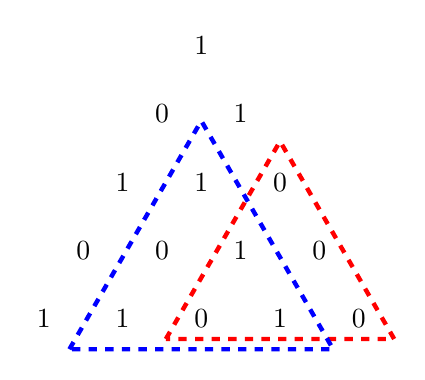
\begin{tikzpicture}
    \node at (0, 0) {1};
    \node at (1, 0) {1};
    \node at (2, 0) {0};
    \node at (3, 0) {1};
    \node at (4, 0) {0};
    \node at (0 + 0.5, {1 * sqrt(3)/2}) {0};
    \node at (1 + 0.5, {1 * sqrt(3)/2}) {0};
    \node at (2 + 0.5, {1 * sqrt(3)/2}) {1};
    \node at (3 + 0.5, {1 * sqrt(3)/2}) {0};
    \node at (0 + 1, {2 * sqrt(3)/2}) {1};
    \node at (1 + 1, {2 * sqrt(3)/2}) {1};
    \node at (2 + 1, {2 * sqrt(3)/2}) {0};
    \node at (0 + 1.5, {3 * sqrt(3)/2}) {0};
    \node at (1 + 1.5, {3 * sqrt(3)/2}) {1};
    \node at (0 + 2, {4 * sqrt(3)/2}) {1};

    % \foreach \t in {1.5} {
    \def\t {1.3};
    \draw[red, ultra thick, dashed]
      ({2 + (1 - \t) * 1.5}, {(1 - \t) * sqrt(3)/2})--
      ({2 + (1 - \t) * 1 + \t * 1}, {\t * sqrt(3)})--
      ({2 + (1 - \t) * 0.5 + \t * 2}, {(1 - \t) * sqrt(3)/2})--
      ({2 + (1 - \t) * 1.5}, {(1 - \t) * sqrt(3)/2});

      \def\t {1.45};
      \draw[blue, ultra thick, dashed]
        ({1 + (1 - \t) * 1.5}, {(1 - \t) * sqrt(3)/2})--
        ({1 + (1 - \t) * 1 + \t * 1}, {\t * sqrt(3)})--
        ({1 + (1 - \t) * 0.5 + \t * 2}, {(1 - \t) * sqrt(3)/2})--
        ({1 + (1 - \t) * 1.5}, {(1 - \t) * sqrt(3)/2});
    \end{tikzpicture}
    \caption{
      On the left is an example of a triangle on two labels that has no
      sub-triangles with equal corners. On the right is a non-example of such a
      triangle on two labels---it has two sub-triangles with equal corners.
    }
\end{figure}

\begin{question}
  Given $n$ labels, what is the biggest triangle that can be constructed?
  Call the side length of such a triangle $a(n)$.
\end{question}
\begin{related}
  \item Given a triangle of side length $k$ and labels up to $n$, what number
    of sub-triangles with equal corners must exist?
  \item How many such triangles exist?
  \item What if any orientation of equilateral triangles are not allowed to have equal corners?
  \item What if this is done with hexagons instead of triangles?
  \item What if this is done on a square grid?
  \item What if for $n \geq 3$ no two corners are allowed to be equal?
\end{related}
\begin{references}
  \item \url{https://math.stackexchange.com/a/2416790/121988}
  \item \url{https://math.stackexchange.com/a/2636168/121988}
\end{references}
\end{document}
